\section{Axiom 3 (Local Commutativity)}\label{sctn:axiom-3-(local-commutativity)}
So far the axioms have differed little from those of AQFT in Minkowski spacetime. This ceases to be true for subsequent axioms. The primary reason for this is that the existence of a quasilocal algebra is not guaranteed on a Lorentzian spacetime. Let us prove this is the case.

\subsection{Quasilocal Algebra?}
Naively, to define a quasilocal algebra associated with a Lorentzian spacetime $M$ one would first consider the set-theoretic union of all $\mathfrak{U}(\mathbf{B})$ over all basis elements $\mathbf{B}$ of the Alexandrov topology on $M$ and prove this set-theoretic union is a normed *-algebra. It turns out that for a generic Lorentzian spacetime $M$ this set-theoretic union isn't a normed *-algebra and thus the construction of the quasilocal algebra fails. Let's see why this is the case.

Consider $M_{BH}$ the Schwarzschild blackhole solution Lorentzian spacetime. $M_{BH}$ has the following Penrose diagram
\begin{figure}[h]
    \centering
    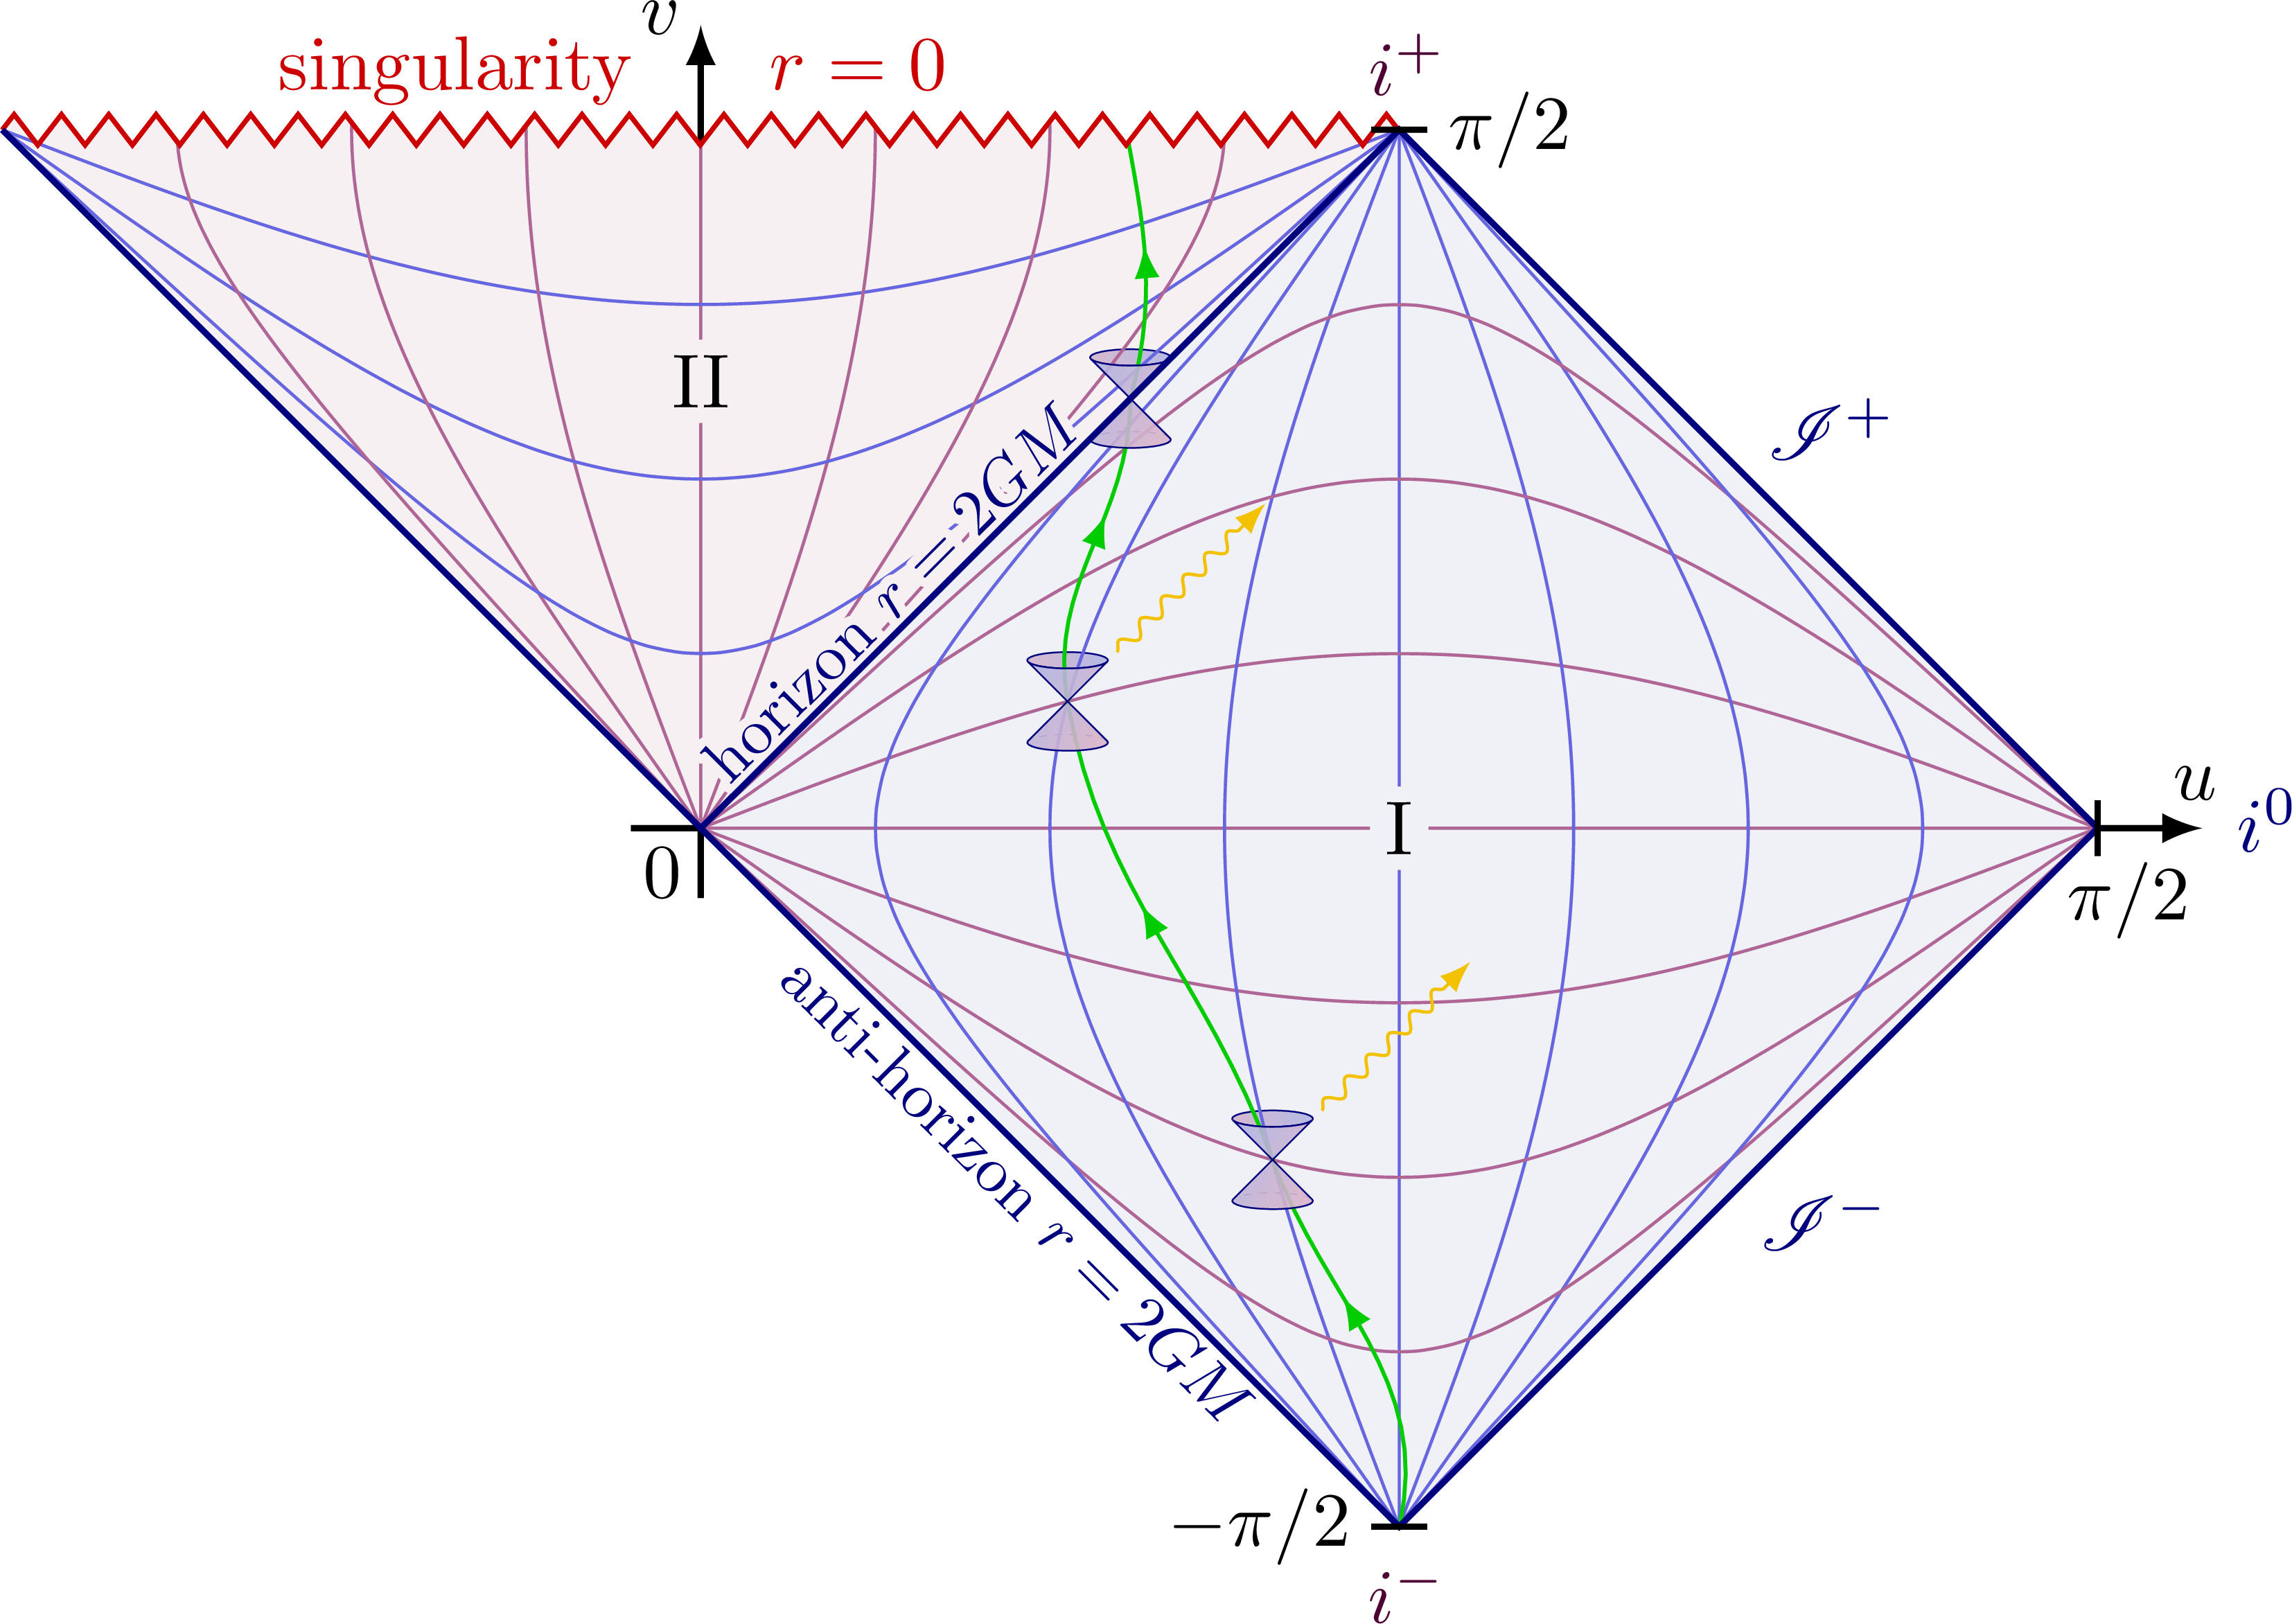
\includegraphics[alt={{Penrose diagram of the Schwarzschild blackhole solution}}, width=\linewidth]{images/schwarzschild_penrose_diagram.png}
\end{figure}
Zooming in on the singularity we can introduce two basis elements $\mathbf{B}_1$ and $\mathbf{B}_2$ of the Alexandrov topology one of which is ``$\varepsilon$ from the singularity'' and the second of which is ``$\varepsilon$ from $i^+$"
\begin{figure}[h]
    \centering
    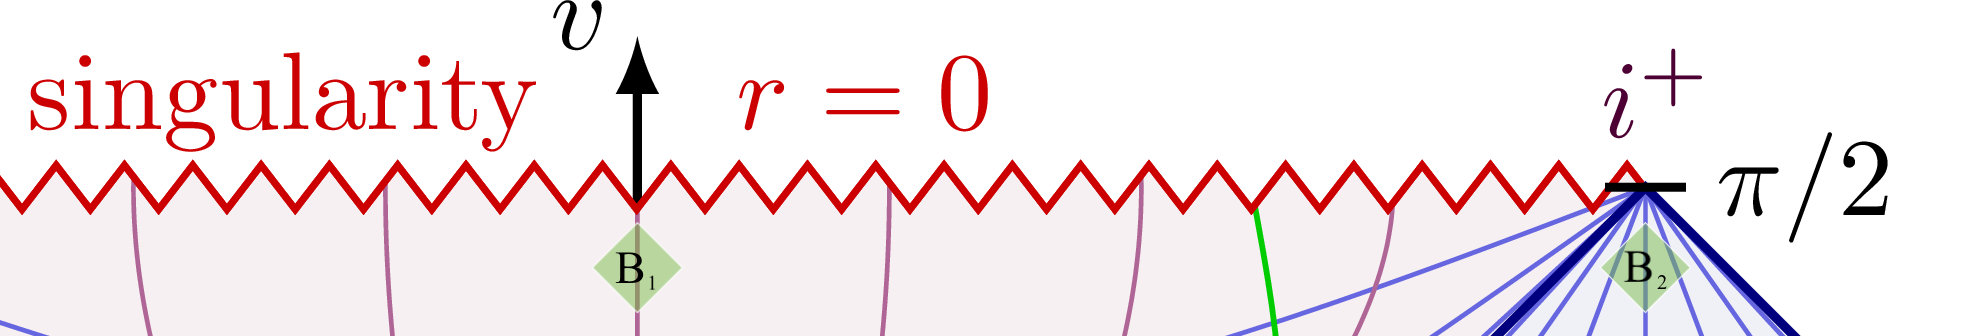
\includegraphics[alt={{Penrose diagram of the Schwarzschild blackhole solution zoomed to singularity, and containing two basis elements}}, width=\linewidth]{images/schwarzschild_penrose_diagram_zoom1.png}
\end{figure}
What is obvious is that there exists no basis element $\mathbf{B}$ of the Alexandrov topology that contains both $\mathbf{B}_1$ and $\mathbf{B}_2$ as it would have to extend beyond the singularity off of $M_{BH}$ which is of course not allowed.

As a result of this, one can not employ the isotony axiom, the only tool one has, to place $\mathfrak{U}(\mathbf{B}_1)$ and $\mathfrak{U}(\mathbf{B}_2)$ in a larger algebra, an algebra in which addition and multiplication of their elements would make sense.

This implies that the set-theoretic union of all $\mathfrak{U}(\mathbf{B})$ over all basis elements $\mathbf{B}$ of the Alexandrov topology on $M_{BH}$ is not a normed *-algebra. This in turn implies that the construction of the quasilocal algebra fails\footnote{This argument can be formalized. However, doing so doesn't provide any insight beyond what's presented by this informal argument. Hence, we omitted the formal argument.} for $M_{BH}$.

For any two basis elements $\mathbf{B}_1$ and $\mathbf{B}_2$ of the Alexandrov topology on a generic Lorentzian spacetime $M$ the best one can hope for is that there exists a third element $\mathbf{B}$ of the Alexandrov topology such that $\mathbf{B}_1, \mathbf{B}_2 \subseteq \mathbf{B}$. However, there is no guarantee that such a $\mathbf{B}$ exists in a Lorentzian spacetime.

All that being said, we can still state a variation of Axiom 3 (Local Commutativity) that applies to a Lorentzian spacetime.

\subsection{Axiom 3 (Local Commutativity)}
The variation of Axiom 3 (Local Commutativity) as applied to Lorentzian spacetime is the following:

\begin{axiom}[Local Commutativity]
    Let $\mathbf{B}_1$ and $\mathbf{B}_2$ be any two basis elements of the Alexandrov topology on a Lorentzian spacetime, i.e. any two sets of the form $I^+(p_1) \cap I^-(q_1)$ and $I^+(p_2) \cap I^-(q_2)$.
    
    If $\mathbf{B_1}$ and $\mathbf{B_2}$ are completely spacelike, for any basis element $\mathbf{B}$ such that $\mathbf{B_1}, \mathbf{B_2} \subseteq \mathbf{B}$ the algebras $\mathfrak{U}(\mathbf{B_1})$ and $\mathfrak{U}(\mathbf{B_2})$ commute in the C*-algebra $\mathfrak{U}(\mathbf{B})$, i.e. for any $a_1$ in $\mathfrak{U}(\mathbf{B_1})$ and $a_2$ in $\mathfrak{U}(\mathbf{B_2})$ we have
    \begin{align}
        i(a_1) i(a_2) - i(a_2) i(a_1) = 0
    \end{align}
    in the C*-algebra $\mathfrak{U}(\mathbf{B})$, where $i$ is the unital *-monomorphism Axiom 2 (Isotony).
    
    If no such $\mathbf{B}$ exists, then it simply doesn't make sense to consider if $\mathfrak{U}(\mathbf{B_1})$ and $\mathfrak{U}(\mathbf{B_2})$ commute as they are not in the same algebra.
\end{axiom}

While having the commutation status of $\mathfrak{U}(\mathbf{B_1})$ and $\mathfrak{U}(\mathbf{B_2})$ sometimes being undefined seems ``odd'' at first. It's actually not ``odd'' at all. The commutation status of $\mathfrak{U}(\mathbf{B_1})$ and $\mathfrak{U}(\mathbf{B_2})$ is only undefined when it's impossible to conduct an experiment that determines if they commute. This makes complete sense.
